\chapter{PHÂN TÍCH ĐỀ TÀI VÀ PHƯƠNG ÁN THIẾT KẾ}
\section{Thông số thiết kế}

\begin{center}
    \begin{figure}[ht]
    \begin{center}
     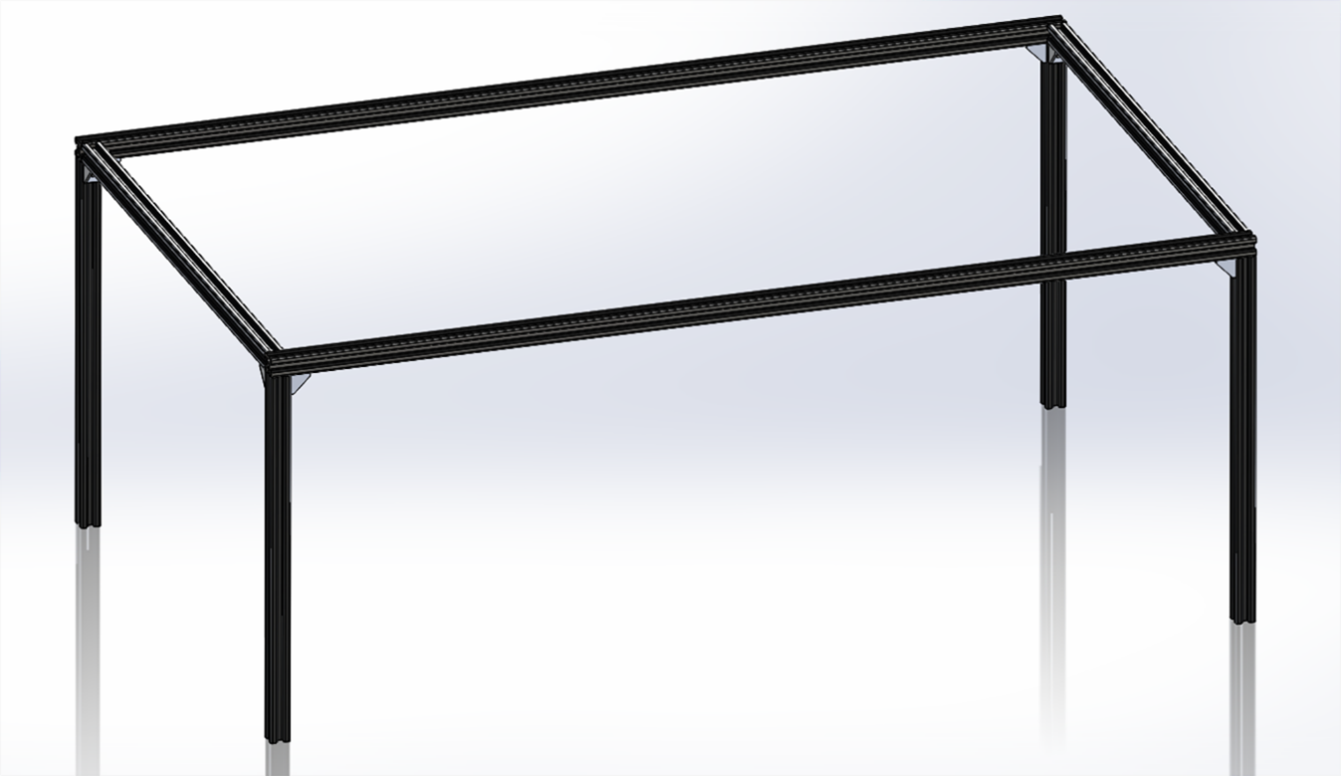
\includegraphics[scale=1]{Chapters/Chapter3/Images/Khungnhomdinhhinh}
    \end{center}
    \caption{Khung nhôm định hình}
    \label{fig:khungnhom}
    \end{figure}
\end{center}

Kích thước khung: 1000 x 600 x 400 mm (dài x rộng x cao).

\section{Phương hướng và giải pháp thực hiện}
Để thiết kế được hệ thống đèn có thể điều chỉnh để nhầm ứng cường độ sáng tại các điểm, ta cần giải quyết được các vấn đề:
\begin{itemize}
\item Tịnh tiến được các dàn đèn
\item Điều khiển dễ dàng, chính xác.
\item Không gây tiếng ồn đáng kể.
\end{itemize}

Dựa theo đó, ta có các phương án sau:

\subsection{Phương án 1}
Ta tịnh tiến các dàn đèn bằng chuyển động trượt, dùng các con lăn nhôm V-slot trượt trên nhôm (Hình~\ref{fig:phuongan1}).
\begin{center}
    \begin{figure}[ht]
    \begin{center}
     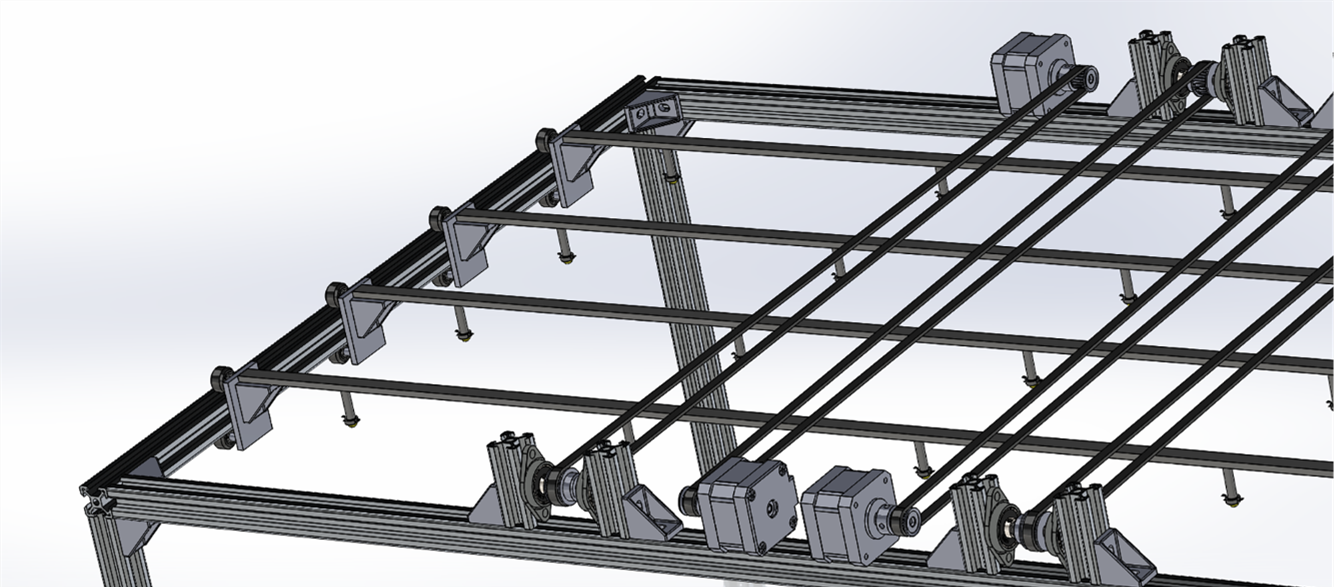
\includegraphics[scale=1]{Chapters/Chapter3/Images/Phuongan1}
    \end{center}
    \caption{Phương án 1}
    \label{fig:phuongan1}
    \end{figure}
\end{center}

\subsection{Phương án 2}
Ta tịnh tiến các dàn đèn bằng chuyển động trượt, dùng 2 con trượt vuông chuyển động trên ti trượt (Hình~\ref{fig:phuongan2}). 
\begin{center}
    \begin{figure}[htp]
    \begin{center}
     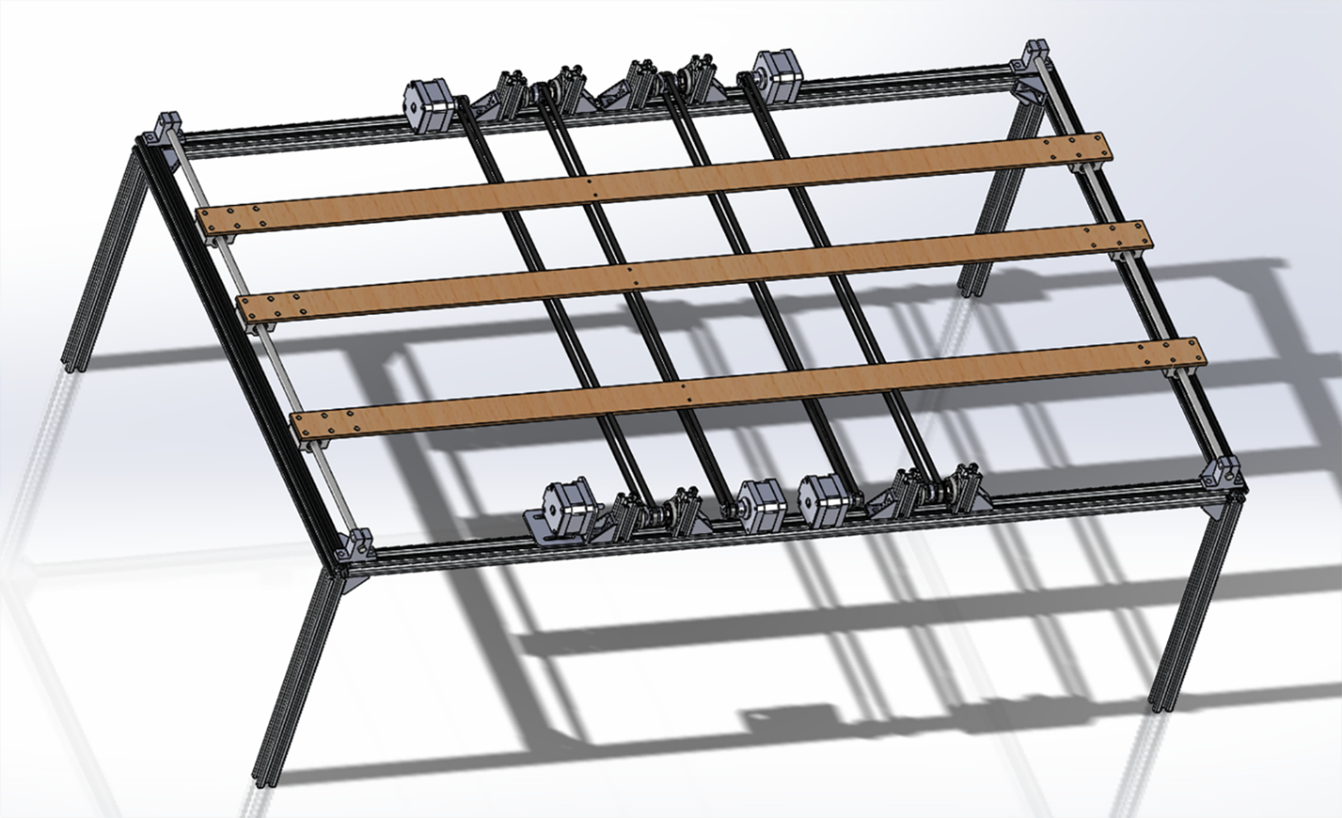
\includegraphics[scale=1]{Chapters/Chapter3/Images/Phuongan2}
    \end{center}
    \caption{Phương án 2}
    \label{fig:phuongan2}
    \end{figure}
\end{center}

\subsection{Phương án 3}
Ta tịnh tiến các dàn đèn bằng chuyển động trượt, dùng 2 con trượt vuông chuyển động trên ti trượt (Hình~\ref{fig:phuongan3}). 
\begin{center}
    \begin{figure}[htp]
    \begin{center}
     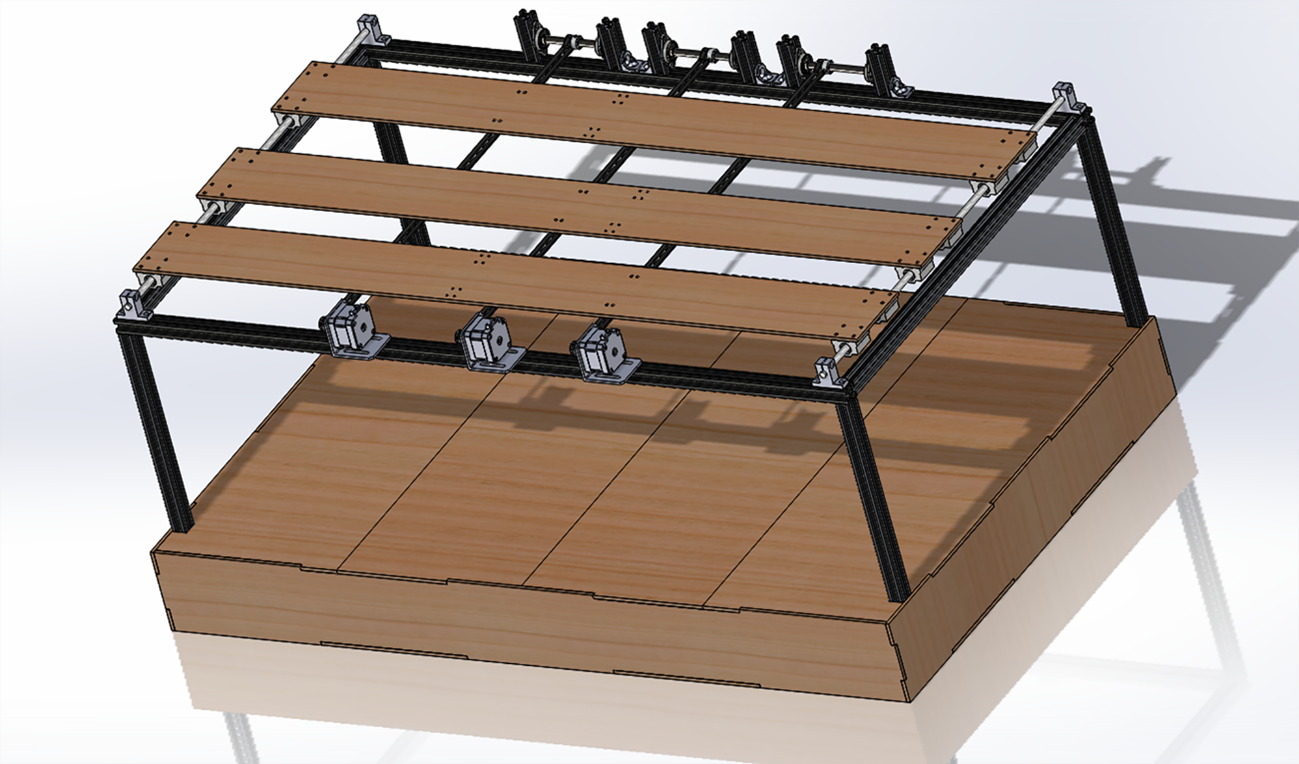
\includegraphics[scale=1]{Chapters/Chapter3/Images/Phuongan3}
    \end{center}
    \caption{Phương án 3}
    \label{fig:phuongan3}
    \end{figure}
\end{center}

\subsection{Lựa chọn phương án tối ưu:}

\begin{table}[H]
\centering
\begin{tabular}{|c|c|c|c|}
\hline 
Đặc điểm & Phương án 1 & Phương án 2 & Phương án 3 \\ 
\hline 
Ổn định & + & - & + \\ 
\hline 
Chi phí & - & + & + \\ 
\hline 
Chính xác & - & - & + \\ 
\hline 
Cơ cấu đơn giản & - & + & + \\ 
\hline 
Khả năng lắp ráp, thay thế & + & + & + \\ 
\hline 
Không gian hoạt động & + & + & - \\ 
\hline 
\textbf{Tổng} & 3+ & 4+ & 5+ \\ 
\hline 
\end{tabular} 
\caption{So sánh các phương án thiết kế cơ cấu truyền động}
\label{tab:sosanhcokhi}
\end{table}

Sau khi so sánh ưu nhược điểm của từng phương án, nhóm quyết định lựa chọn phương án 3. (Bảng \ref{tab:sosanhcokhi})

\section{Chọn động cơ}
\begin{table}[H]
\centering
\begin{tabular}{|c|p{5.5cm}|p{5.5cm}|}
\hline
 & Động cơ STEP & Động cơ DC Servo \\
\hline 
Ưu điểm & 
- Tạo ra chuyển động gia tăng, giảm chi phí và độ phức tạp của bộ mã hóa.

- Số cực cao nên có thể tạo ra mô-men xoắn rất cao ở tốc độ 0.

- Kích thước nhỏ gọn, tiết kiệm chi phí.
& 
- Là hệ thống hồi tiếp vòng kín chính vì vậy động cơ servo DC rất dễ điều khiển, dễ sử dụng.

- Mô-men xoắn khởi động lớn.

- Có thể được sử dụng trong các ứng dụng công nghiệp và dân dụng nói chung nhạy cảm với chi phí. \\ 
\hline 
Nhược điểm & 
- Tốc độ bị giới hạn, chạy tốt nhất ở 1200 vòng/phút hoặc thấp hơn.

- Mặc dù tạo mô-men xoắn cao ở tốc độ 0, nhưng mô-men xoắn sẽ rơi khi tốc độ tăng.
 & 
- Vì cấu tạo có bộ phận chổi than nên điểm hạn chế lớn nhất của loại động cơ này chính là dễ gây ra tiếng ồn, nhiệt độ cao.

- Quán tính cao khi giảm tốc độ.

- Bảo trì bất tiện (thay thế chổi than). \\ 
\hline 
\end{tabular} 
\caption{Bảng so sánh động cơ Step và động cơ DC Servo}
\label{tab:sosanhdongco}
\end{table}

Trong kỹ thuật không có giải pháp nào hoàn hảo, mà chỉ được coi là giải pháp tốt nhất, đặc biệt đối với động cơ SERVO và động cơ STEP. Cả hai đều được sử dụng rộng rãi trong ngành công nghiệp. Khi được áp dụng đúng cách, hai động cơ này đều có thể mang lại hiệu quả làm việc đáng mong đợi cho cả hệ thống máy. Để đi tới quyết định lựa chọn loại động cơ nào phù hợp thì phụ thuộc vào rất nhiều yếu tố, nhưng quan trọng nhất là tốc độ, gia tốc và giá cả.


Vì trong đề tài này, nhóm thực hiện mô hình với kích thước nhỏ, với mục đích điều khiển dễ dàng, chính xác và không gây tiếng ồn với chi phí thấp, dễ thay thế, bảo trì nên qua việc phân tích những ưu điểm và nhược điểm của hai loại động cơ này (Bảng~\ref{tab:sosanhdongco}), ta thấy động cơ STEP sẽ phù hợp với mô hình hơn.

\textbf{Động cơ bước NEMA17:} (Hình~\ref{fig:nema17})
\begin{center}
    \begin{figure}[htp]
    \begin{center}
     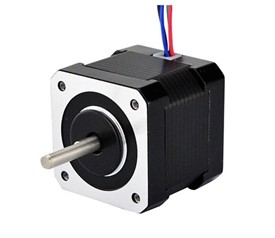
\includegraphics[scale=1]{Chapters/Chapter3/Images/NEMA17}
    \end{center}
    \caption{Động cơ bước NEMA17}
    \label{fig:nema17}
    \end{figure}
\end{center}
\begin{table}[H]
\centering
\begin{tabular}{|p{0.12\linewidth}|p{0.12\linewidth}|p{0.12\linewidth}|p{0.12\linewidth}|p{0.12\linewidth}|p{0.12\linewidth}|p{0.12\linewidth}|p{0.12\linewidth}|}
\hline 
Động cơ bước & Kích thước motor ($mm$) & Bước góc ($^{\circ}$) & Cường độ dòng điện ($A$) & Điện trở pha ($\Omega$) & Moment xoắn ($Nmm$) & Moment quán tính ($g.cm^2$) & Trọng lượng ($g$) \\
\hline 
NEMA 17 & $42x42$ & 1.8 & 1.7 & 5.75 & 280 & 100 & 300 \\
\hline 
\end{tabular} 
\caption{Bảng thông số kỹ thuật của động cơ NEMA17}
\label{tab:NEMA17}
\end{table}

\section{Lựa chọn các chi tiết cho mô hình}

\textbf{Nhôm định hình:} nhóm đã sử dụng nhôm định hình 20 x 20 để làm khung. (Hình~\ref{fig:nhomdinhhinh})

Ưu điểm:
\begin{itemize}
\item Có kết cấu vững chắc, bền vững với thời gian.
\item Không bị cong vênh, không bị oxi hóa, không biến đổi do nhiệt.
\item Ưu điểm vượt trội về khối lượng cũng như không bị mối mọt như gỗ.
\item Được sơn tĩnh điện, không bị bong sơn, tính thẩm mĩ cao.
\end{itemize}
\begin{center}
    \begin{figure}[htp]
    \begin{center}
     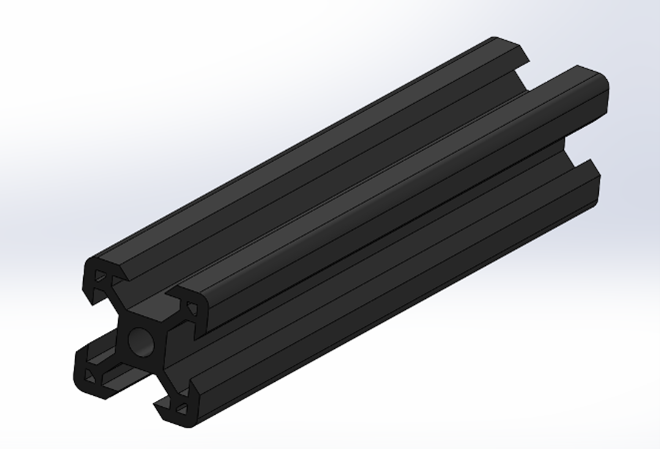
\includegraphics[scale=1]{Chapters/Chapter3/Images/Nhomdinhhinh}
    \end{center}
    \caption{Nhôm định hình 20x20}
    \label{fig:nhomdinhhinh}
    \end{figure}
\end{center}

\textbf{Ke góc vuông:} Ke sử dụng để cố định và gá các thanh nhôm tạo khung. (Hình~\ref{fig:kegocvuong})
\begin{center}
    \begin{figure}[htp]
    \begin{center}
     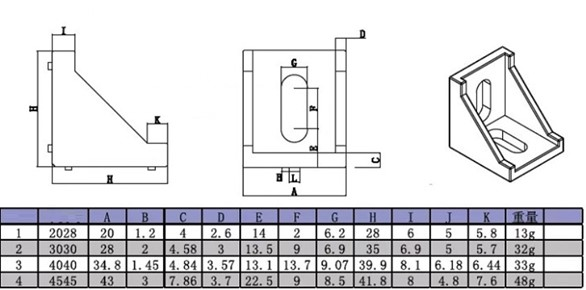
\includegraphics[scale=1]{Chapters/Chapter3/Images/Kegocvuong}
    \end{center}
    \caption{Ke góc vuông}
    \label{fig:kegocvuong}
    \end{figure}
\end{center}

\textbf{Gối đỡ trục:} Gối đỡ thanh trượt tròn 8mm dùng đỡ 2 đầu cho các thanh trượt tròn. (Hình~\ref{fig:goidotruc})
\begin{center}
    \begin{figure}[htp]
    \begin{center}
     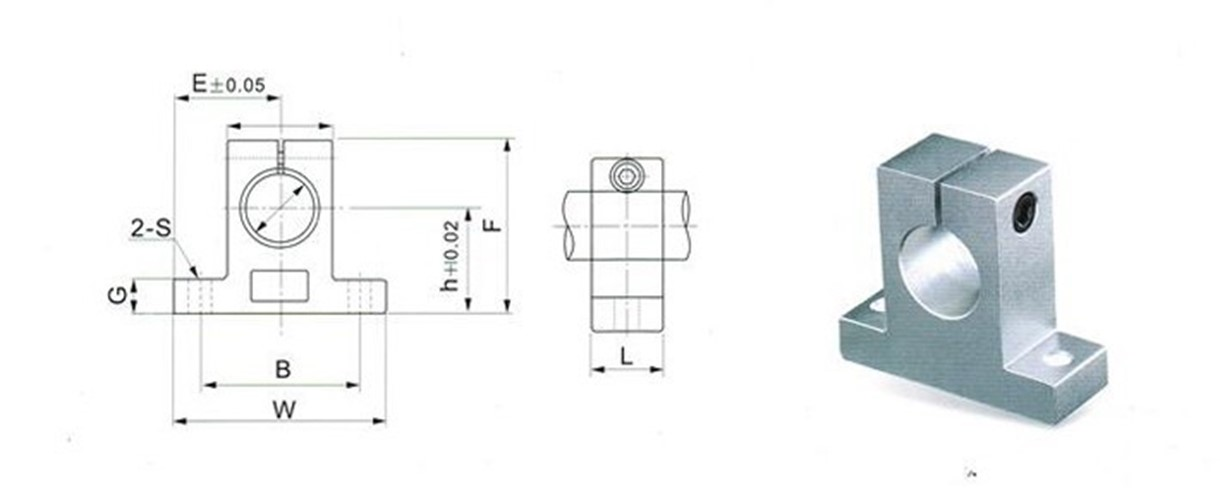
\includegraphics[scale=1]{Chapters/Chapter3/Images/Goidotruc}
    \end{center}
    \caption{Gối đỡ trục}
    \label{fig:goidotruc}
    \end{figure}
\end{center}
\begin{center}
    \begin{figure}[htp]
    \begin{center}
     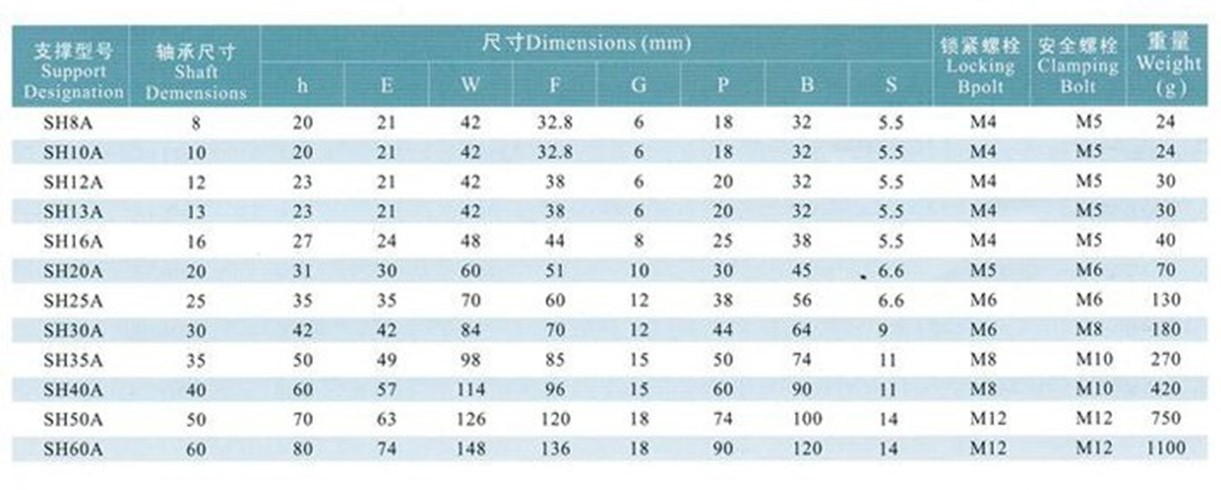
\includegraphics[scale=1]{Chapters/Chapter3/Images/Kichthuocgoidotruc}
    \end{center}
    \caption{Bảng kích thước gối đỡ trục}
    \label{fig:kichthuocgoidotruc}
    \end{figure}
\end{center}

\textbf{Con trượt vuông:} cho phép các chi tiết máy móc chuyển động tinh tiến chính xác, mượt mà, nhẹ nhàng, êm ái, ít lực ma sát nhất. (Hình~\ref{fig:contruotvuong})
\begin{center}
    \begin{figure}[htp]
    \begin{center}
     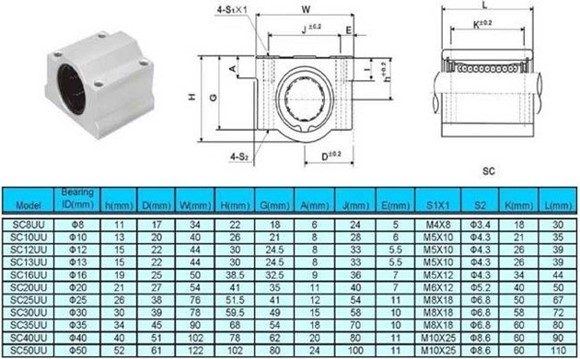
\includegraphics[scale=1]{Chapters/Chapter3/Images/Contruotvuong}
    \end{center}
    \caption{Con trượt vuông}
    \label{fig:contruotvuong}
    \end{figure}
\end{center}

\textbf{Gối đỡ vòng bi ngang:} (Hình~\ref{fig:goidovongbingang})

\begin{center}
    \begin{figure}[htp]
    \begin{center}
     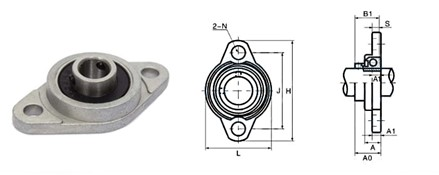
\includegraphics[scale=1]{Chapters/Chapter3/Images/Goidovongbingang}
    \end{center}
    \caption{Gối đỡ vòng bi ngang}
    \label{fig:goidovongbingang}
    \end{figure}
\end{center}

\textbf{Puly:} Pully có lỗ 5mm tương thích với đa số các động cơ bước, đặc biệt loại động cơ bước NEMA17. (Hình~\ref{fig:puly})
\begin{center}
    \begin{figure}[htp]
    \begin{center}
     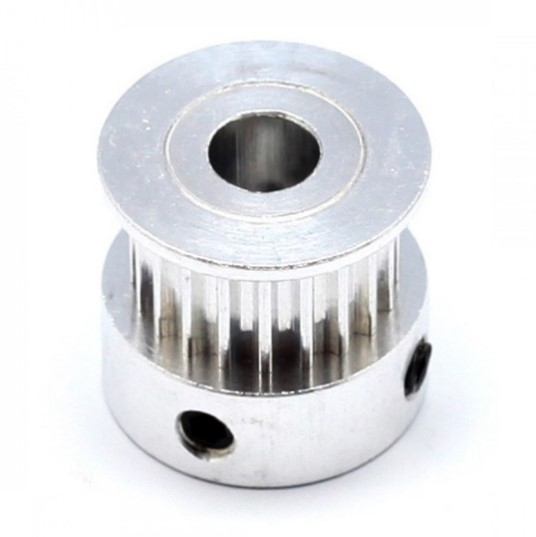
\includegraphics[scale=0.7]{Chapters/Chapter3/Images/Puly}
    \end{center}
    \caption{Puly trục 5mm 20 răng}
    \label{fig:puly}
    \end{figure}
\end{center}

\textbf{Dây đai GT2:} sử dụng profin bo tròn, bước răng 2mm đảm bảo các răng của đai khít vừa vặn và chính xác. (Hình~\ref{fig:daiGT2})
\begin{center}
    \begin{figure}[htp]
    \begin{center}
     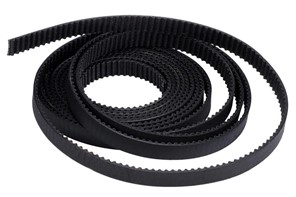
\includegraphics[scale=0.7]{Chapters/Chapter3/Images/DaiGT2}
    \end{center}
    \caption{Dây đai GT2}
    \label{fig:daiGT2}
    \end{figure}
\end{center}
\clearpage
\section{Tính toán lựa chọn đèn}
Vấn đề chiếu sáng trong văn phòng, trong các phòng kín luôn là vấn đề được nghiên cứu và phát triển. Mục đích chiếu sáng tạo ra môi trường ánh sáng tốt, tiện nghi, làm cho người sử dụng cảm thấy dễ chịu. Ngoài ra ở các giảng đường, thư viện hay các văn phòng kín , việc chiếu sáng giúp cho người học hay người làm cảm thấy làm việc học tập có hiệu quả hơn.

Yêu cầu của đèn khi thiết kế cần đảm bảo:
\begin{itemize}
\item Đảm bảo được độ rọi để phục vụ cho công việc, việc học tập.
\item Đảm bảo tiện nghi, không gây lóa mắt.
\item Màu sắc và nhiệt độ trong phòng phù hợp.
\item Vấn đề thẩm mỹ và tiết kiệm năng lượng.	
\end{itemize}

\subsection{Chọn độ rọi}
Độ rọi của đèn thể hiện được bề mặt làm việc, nơi đó còn gọi là “bề mặt hữu ích” với mô hình nhóm lựa chọn có độ cao là 300mm so với mặt sàn.

 Độ rọi này phụ thuộc vào góc chiếu của đèn, của chóa đèn….ở cấp độ mô hình thì nhóm mong muốn là giữa các phần giao thoa của đèn thì cường độ ánh sáng được đảm bảo với cường độ ánh sáng mong muốn.
 
 Hình \ref{fig:doroi} thể hiện ảnh hưởng của ánh sáng tự nhiên vào căn phòng, có thể thấy ở các vùng gần cửa sổ thì có cường độ ánh sáng cao nhưng ở nơi xa cửa sổ (trung tâm phòng học) có cường độ thấp hơn.

\subsection{Chọn loại đèn}
Việc lựa chọn đèn thích hợp nhất trong các loại đèn được nhóm triển khai theo các tiêu chuẩn sau đây:
\begin{itemize}
\item Góc chiếu của đèn đảm bảo được các vùng sáng giao thoa nhau.
\item Đèn có cường độ ánh sáng có thể điều chỉnh phù hợp.
\item Tuổi thọ của đèn.
\item Hiệu quả ánh sáng của đèn.
\item Chi phí.
\end{itemize}

\begin{center}
    \begin{figure}[ht]
    \begin{center}
     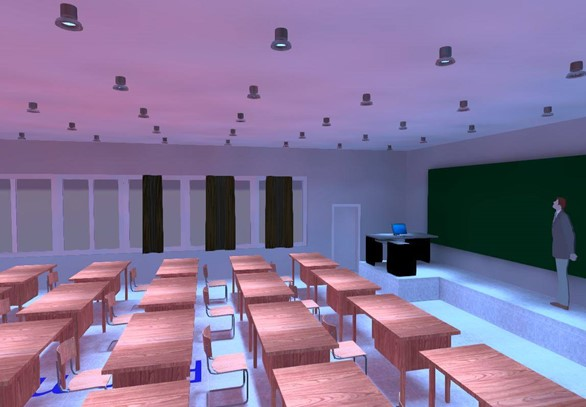
\includegraphics[scale=1]{Chapters/Chapter3/Images/Phonghocmophong}
    \end{center}
    \caption{Mô phỏng bố trí đèn chiếu trong phòng học sử dụng phần mềm DIALux}
    \label{fig:phonghocmophong}
    \end{figure}
\end{center}

\subsection{Chọn phương án chiếu sáng và bộ đèn}
Trong cuộc sống chúng ta thường gặp những cách chiếu sáng trực tiếp và bán trực tiếp. Kiểu chiếu sáng phụ thuộc vào các yếu tố ngoại quan như ánh sáng môi trường, thời tiết, khí hậu, tính phản xạ,…

Đối với loại đèn khác nhau, thì nhà sản xuất đã cung cấp catalog cho phép chọn kiểu bộ đèn, cấp xác định và nếu có thể người sản xuất đảm bảo có đủ các loại công suất khác nhau.

\subsection{Bố trí các đèn}
Không gian của nhóm thực hiện là không gian hình chữ nhật nên nhóm lựa chọn phương án bố trí đèn theo từng dàn cách đều nhau.

Bằng cách tính tổng quan thông số của đèn thì ta tính được số đèn tương ứng để chiếu sáng. Vì thế số đèn chọn là nhỏ nhất nhưng bố trí đều đặn sao cho khi sử dụng thì đèn sẽ đồng đều và độ rọi sẽ tốt nhất.

\subsection{Thực nghiệm và chọn loại đèn phù hợp}
Sau khi tìm hiểu các yêu cầu mà bóng đèn cần có thì nhóm đã tiến hành mô phỏng tính toán để chọn ra các loại đèn tối ưu nhất đáp ứng các nhu cầu đề ra và tiến hành lắp ráp thực tế. Các loại đèn được nhóm lựa chọn: đèn công suất siêu sáng 3W, 5W, 10W.


\textbf{Đèn LED công suất 10W:} (Hình~\ref{fig:10W})

Đèn siêu sáng 10W cung cấp ánh sáng trắng với cường độ cao có thể thay đổi được, trong khi thực tiễn thì mặc dù đáp ứng được độ sáng cho mô hình nhưng vẫn còn tồn tại rất nhiều nhược điểm như:

\begin{itemize}
\item Bóng tỏa một lượng nhiệt rất lớn.
\item Công suất tiêu thụ lớn.
\item Giá thành của bóng cao.
\item Việc điều khiển cường độ ánh sáng ở chế độ auto thì gặp nhiều cản trở do góc chiếu của đèn khá rộng.
\end{itemize}
\begin{center}
    \begin{figure}[ht]
    \begin{center}
     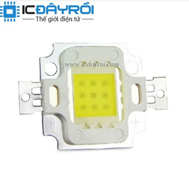
\includegraphics[scale=1]{Chapters/Chapter3/Images/Led10W}
    \end{center}
    \caption{Đèn LED công suất 10W}
    \label{fig:10W}
    \end{figure}
\end{center}

\textbf{Đèn LED công suất 5W:} (Hình~\ref{fig:5W})

Led 5W cung cấp ánh sáng trắng cho toàn bộ căn phòng, thỏa mãn các điều kiện cần của mô hình nhưng vẫn còn tồn tại là giá thành cao, và khi không có các yếu tố bên ngoài thì ánh sáng của led khi hoạt động ở trạng thái 100\% thì vẫn vượt quá mức cần thiết rất nhiều.
\begin{center}
    \begin{figure}[ht]
    \begin{center}
     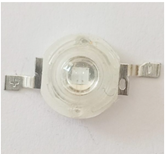
\includegraphics[scale=1]{Chapters/Chapter3/Images/Led5W}
    \end{center}
    \caption{Đèn LED công suất 5W}
    \label{fig:5W}
    \end{figure}
\end{center}

\textbf{Đèn LED công suất 3W:} (Hình~\ref{fig:3W})

Led siêu sáng 3W cho cường độ ánh sáng với góc chiếu tính toán đạt yêu cầu. giá thành của đèn thì là rẻ nhất trong các loại đèn được nhóm đưa ra lựa chọn. Tuy còn điểm yếu chung là góc chiếu nhóm cần tìm và thiết kế chóa phù hợp với đèn.
\begin{center}
    \begin{figure}[ht]
    \begin{center}
     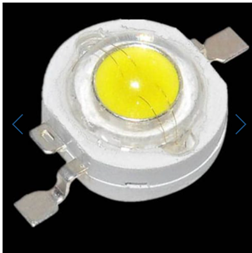
\includegraphics[scale=1]{Chapters/Chapter3/Images/Led3W}
    \end{center}
    \caption{Đèn LED công suất 3W}
    \label{fig:3W}
    \end{figure}
\end{center}

Như vậy qua việc tìm hiểu và kiểm thử các loại đèn thì nhóm chọn được đèn phù hợp với đồ án của nhóm là led siêu sáng 3W với chóa đèn do nhóm tự thiết kế.
